\documentclass[conference]{IEEEtran}
\IEEEoverridecommandlockouts

\usepackage{cite}
\usepackage{amsmath}
\usepackage{fontspec}
\usepackage{unicode-math}
\setmainfont{texgyretermes}[Extension=.otf, UprightFont=*-regular, BoldFont=*-bold,
  ItalicFont=*-italic, BoldItalicFont=*-bolditalic]
\setmathfont{texgyretermes-math.otf}
\usepackage{graphicx}
\usepackage{booktabs}
\usepackage{xurl}
\usepackage{xcolor}
\usepackage{siunitx}
\sisetup{group-separator={,}, group-minimum-digits=4}

\begin{document}

\title{WattToWater: Measuring and Comparing the Water\\Footprint of Compute Workloads}

\author{\IEEEauthorblockN{G\"{o}zde G\"{o}n\"{u}l}
\IEEEauthorblockA{Independent Researcher\\
T\"{u}rkiye}}

\maketitle

\begin{abstract}
The same compute job can need 6.7 times more water in one data-center region than in another, and the region with the fewest litres is not always the one with the least water stress. We present WattToWater, an open prototype that converts the energy used by a software job into litres of water and compares the result across 11 data-center regions. Water is split into on-site cooling water and off-site water used to generate electricity, using published regional factors. Energy is estimated from CPU utilisation on a laptop. For a 200-tree Random Forest training run ($5.96\times10^{-5}$~kWh), the water footprint ranges from 0.106~mL (Ireland) to 0.708~mL (Washington). Off-site water is at least 78\% of the total in every region. Litres and water stress rank regions differently: Texas has the second-lowest footprint but High baseline water stress, while Washington has the highest footprint but only Low--Medium stress. We therefore report both side by side. A second experiment shows that the model itself is a lever: 100 trees used 48\% of the energy and water of 200 trees at the same test accuracy (96.15\% vs.\ 95.90\%). Energy is an estimate with stated assumptions, so the results illustrate the method and do not measure any real facility.
\end{abstract}

\begin{IEEEkeywords}
water footprint, data centers, sustainable computing, green AI, water stress, energy estimation
\end{IEEEkeywords}

\section{Introduction}

Running software uses water in two places. Data centers evaporate water to cool their servers (on-site, or scope~1 water), and power plants use water to generate the electricity those servers draw (off-site, or scope~2 water)~\cite{li2023thirsty}.

Li~\textit{et al.}~\cite{li2023thirsty} estimate that training GPT-3 in Microsoft's U.S.\ data centers consumed about 5.4 million litres of water, of which about \num{700000} litres was on-site, for a training energy of \num{1287}~MWh. They also estimate about 16.9~mL per request at the U.S.\ average, assuming 0.004~kWh of server energy per request.

A developer rarely sees this number for their own code, and two things make it hard to reason about. First, the footprint of the same job depends strongly on where it runs: across the 11 operating regions we use, water per kWh differs by a factor of 6.7. Second, litres are not scarcity: a litre taken in a water-stressed basin matters more than a litre taken where water is plentiful.

The decisions that set this footprint are made by people who never see a water bill: which cloud region to deploy in, which model size to train, when a job is good enough. WattToWater aims to put the water cost in front of them at that moment, in units they can compare. This paper contributes (i)~a transparent, open pipeline from measured CPU utilisation to energy to on-site and off-site water; (ii)~a measurement protocol with repeated runs, logged conditions and documented exclusions; (iii)~side-by-side reporting of litres and WRI Aqueduct baseline water stress~\cite{wri2023aqueduct} for 11 regions; (iv)~a model-size experiment; and (v)~an open library that brings these numbers to developers, teams and organisations.

\section{Method}

\subsection{Water Footprint Model}

The water footprint $W$ (litres) of a job that uses energy $E$ (kWh) in a given region is the sum of an on-site and an off-site term:
\begin{equation}
W = \underbrace{E \cdot \mathrm{WUE}}_{\text{on-site}} + \underbrace{E \cdot \mathrm{PUE} \cdot \mathrm{EWIF}}_{\text{off-site}}
\label{eq:water}
\end{equation}
where WUE is the on-site water usage effectiveness (L per kWh of IT energy), PUE is the power usage effectiveness (total facility energy divided by IT energy), and EWIF is the electricity water intensity factor of the grid (L per kWh of electricity). We take PUE, WUE and EWIF for each region from Table~1 of~\cite{li2023thirsty}, which reports annualised values for Microsoft's data centers (Table~\ref{tab:factors}). We use the 11 regions in that table that were operating; the 7 regions marked as under construction, whose values are projections, are excluded.

\begin{table}[t]
\caption{Regional Water Factors, Sorted by Total Water per kWh}
\label{tab:factors}
\centering
\footnotesize
\setlength{\tabcolsep}{4pt}
\begin{tabular}{@{}lccccc@{}}
\toprule
Region & PUE & WUE & EWIF & Total & On-site \\
 & & (L/kWh) & (L/kWh) & (L/kWh) & share \\
\midrule
Ireland      & 1.19 & 0.02 & 1.476 & 1.78  & 1.1\%  \\
Texas        & 1.28 & 0.25 & 1.287 & 1.90  & 13.2\% \\
Virginia     & 1.14 & 0.14 & 2.385 & 2.86  & 4.9\%  \\
Wyoming      & 1.11 & 0.13 & 2.574 & 2.99  & 4.4\%  \\
Iowa         & 1.16 & 0.14 & 3.104 & 3.74  & 3.7\%  \\
Illinois     & 1.35 & 0.74 & 2.233 & 3.76  & 19.7\% \\
Netherlands  & 1.14 & 0.06 & 3.445 & 3.99  & 1.5\%  \\
U.S. average & 1.17 & 0.55 & 3.142 & 4.23  & 13.0\% \\
Sweden       & 1.16 & 0.09 & 6.019 & 7.07  & 1.3\%  \\
Arizona      & 1.18 & 1.63 & 4.959 & 7.48  & 21.8\% \\
Washington   & 1.15 & 0.95 & 9.501 & 11.88 & 8.0\%  \\
\bottomrule
\end{tabular}

\vspace{2pt}
\parbox{\columnwidth}{\scriptsize PUE, WUE and EWIF from~\cite{li2023thirsty}, Table~1. Total $=\mathrm{WUE}+\mathrm{PUE}\cdot\mathrm{EWIF}$ and on-site share computed by the author.}
\end{table}

\subsection{Energy Estimate}

All measurements ran on one laptop with an Intel Core i5-12450H processor (8 cores, 12 threads) under Windows~11. The machine has no discrete NVIDIA GPU, so GPU power sensors were not available. We estimate power from the average system-wide CPU utilisation $u \in [0,1]$ during a run, read with psutil 7.2.2~\cite{psutil}:
\begin{equation}
P = P_{\mathrm{idle}} + (P_{\mathrm{base}} - P_{\mathrm{idle}})\,u, \qquad E = \frac{P\,t}{3.6\times10^{6}}
\label{eq:power}
\end{equation}
where $P$ is in watts, $t$ is the run time in seconds and $E$ is in kWh. $P_{\mathrm{base}} = 45$~W is the processor base power listed by Intel; the same specification lists a maximum turbo power of 95~W~\cite{intel12450h}. $P_{\mathrm{idle}} = 5$~W is our own assumption, without a source. Because the model is linear in $u$, the average utilisation over a run gives the same energy as sampling it repeatedly.

\subsection{Workload and Measurement Protocol}

The workload is the training of a scikit-learn~\cite{pedregosa2011sklearn} \texttt{RandomForestClassifier} (200 trees, all cores, \texttt{random\_state}~=~42) on a synthetic dataset from \texttt{make\_classification} (\num{20000} samples, 20 features, 10 informative), split 80/20 into training and test data. Only training and scoring are timed; data generation is excluded. The test accuracy is 0.959 for 200 trees and is deterministic for a fixed random seed. Software: Python 3.12.0, scikit-learn 1.3.2, NumPy 1.26.4.

We ran the job in sets of five consecutive runs and logged every run together with a note on the condition (Table~\ref{tab:sets}). Set~2 is excluded as an outlier. It ran about 34\% longer than the same condition in Set~3 and started shortly after the applications had been reopened, which may have caused background load; we did not confirm this cause, and its rows remain in the data file. Within Sets 1, 3 and 4 the run time rises from the first to the fifth run (for example 4.36~s to 5.30~s in Set~1), which fits the processor slowing down as it heats up; we did not test this. The 15 runs of Sets 1, 3 and 4 give an energy of $5.96\times10^{-5} \pm 4.5\times10^{-6}$~kWh (mean $\pm$ sd).

\begin{table}[t]
\caption{Measurement Sets}
\label{tab:sets}
\centering
\footnotesize
\begin{tabular}{@{}clcc@{}}
\toprule
Set & Condition & Duration (s) & Used \\
\midrule
1 & Other applications closed & $4.90 \pm 0.41$ & Yes \\
2 & Development tools open    & $6.56 \pm 0.15$ & No  \\
3 & Development tools open    & $4.79 \pm 0.38$ & Yes \\
4 & Other applications closed & $5.10 \pm 0.32$ & Yes \\
\bottomrule
\end{tabular}
\end{table}

For the model-size experiment we trained forests of 25, 50, 100 and 200 trees, three times each, on the same data split. The order of sizes was reversed in every second round so that warm-up would not favour one size, and the laptop rested 10~s between runs.

\subsection{Water Stress}

We take water stress from the baseline water stress indicator (bws) of WRI Aqueduct 4.0~\cite{wri2023aqueduct}, weighted by total water demand, from the country rankings file \texttt{Aqueduct40\_rankings\_download\_Y2023M07D05.xlsx}. The score runs from 0 to 5, and each score maps to a category (Low, Low--Medium, Medium--High, High, Extremely High). For the Netherlands, Ireland, Sweden and the U.S.\ average we use country-level values; for the U.S.\ states we use state-level values. We do not combine litres and stress into a single index: both are reported next to each other.

\subsection{From Measurement to Decisions}

The method is packaged as an open Python library that puts the water footprint where decisions are made, at three levels:
\begin{itemize}
\item \textit{Developer:} one decorator, \texttt{@track\_water}, measures any function or code block, prints its water per region and appends the run to a log.
\item \textit{Team:} \texttt{python -m watttowater report} turns the log into a Markdown summary; a continuous-integration workflow writes it to the summary page of every pipeline run.
\item \textit{Organisation:} a region ranking under a water-stress policy limit (e.g.\ stress $\le 2$), and a model-size advisor that measures variants of a job and suggests the cheapest one within 0.5 percentage points of the best result.
\end{itemize}
Automated tests check that the library reproduces the numbers reported in this paper.

\section{Results}

\subsection{Water by Region}

For the 200-tree training job, the water footprint ranges from 0.106~mL in Ireland to 0.708~mL in Washington, a 6.7-fold difference (Fig.~\ref{fig:region}). Off-site water from electricity generation is the larger part in every region.

\begin{figure*}[t]
\centering
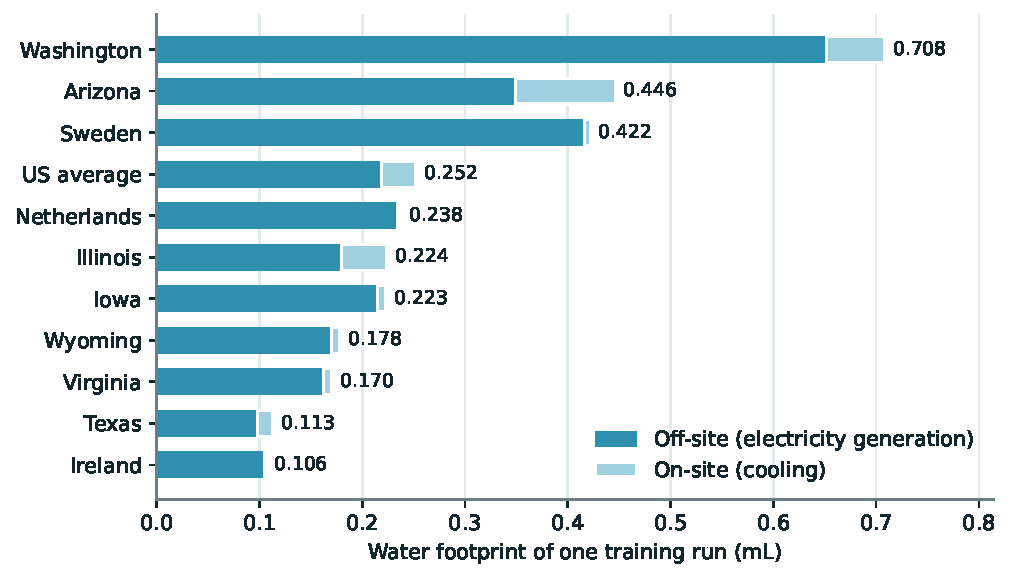
\includegraphics[width=0.66\textwidth]{figures/fig1_water_by_region.pdf}
\caption{Water footprint of one training run per region, split into off-site (electricity generation) and on-site (cooling) water. The same job needs 6.7 times more water in Washington than in Ireland.}
\label{fig:region}
\end{figure*}

\subsection{Litres and Water Stress}

Baseline water stress ranges from 0.36 (Ireland) to 4.39 (Arizona), and it does not follow the litres (Table~\ref{tab:main}, Fig.~\ref{fig:stress}).

\begin{table}[t]
\caption{Water Footprint of One Training Run and Baseline Water Stress}
\label{tab:main}
\centering
\footnotesize
\setlength{\tabcolsep}{5pt}
\begin{tabular}{@{}lccl@{}}
\toprule
Region & Water (mL) & Stress (0--5) & Category \\
\midrule
Ireland$^{*}$      & $0.106 \pm 0.008$ & 0.36 & Low \\
Texas              & $0.113 \pm 0.009$ & 3.33 & High \\
Virginia           & $0.170 \pm 0.013$ & 2.56 & Medium--High \\
Wyoming            & $0.178 \pm 0.014$ & 3.77 & High \\
Iowa               & $0.223 \pm 0.017$ & 1.08 & Low--Medium \\
Illinois           & $0.224 \pm 0.017$ & 2.40 & Medium--High \\
Netherlands$^{*}$  & $0.238 \pm 0.018$ & 1.58 & Low--Medium \\
U.S. average$^{*}$ & $0.252 \pm 0.019$ & 2.60 & Medium--High \\
Sweden$^{*}$       & $0.422 \pm 0.032$ & 0.78 & Low \\
Arizona            & $0.446 \pm 0.034$ & 4.39 & Extremely High \\
Washington         & $0.708 \pm 0.054$ & 1.20 & Low--Medium \\
\bottomrule
\end{tabular}

\vspace{2pt}
\parbox{\columnwidth}{\scriptsize Water: mean $\pm$ sd over 15 runs; the sd covers only run-to-run variation of the measured energy, not the uncertainty of the energy model or the regional factors. Stress: WRI Aqueduct~4.0 bws~\cite{wri2023aqueduct}; $^{*}$country level, others state level.}
\end{table}

\begin{figure*}[t]
\centering
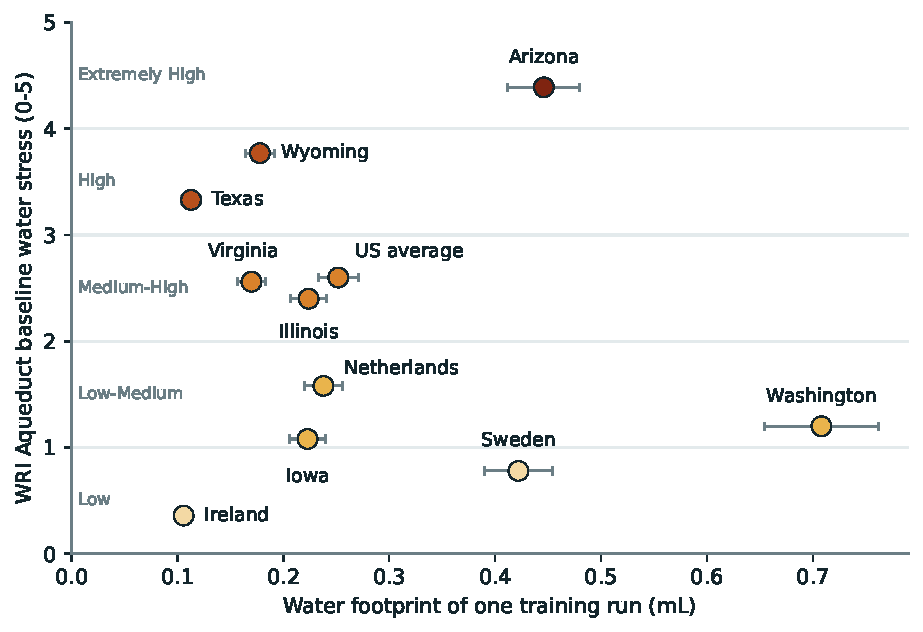
\includegraphics[width=0.54\textwidth]{figures/fig2_water_vs_stress.pdf}
\caption{Water footprint against baseline water stress. Error bars: $\pm1$~sd over 15 runs. Colour follows the Aqueduct stress category.}
\label{fig:stress}
\end{figure*}

\subsection{Model Size}

The size of the model changes the footprint about as much as the choice of region, at almost no cost in accuracy (Table~\ref{tab:trees}, Fig.~\ref{fig:trees}). Energy grew almost exactly in proportion to the number of trees, while accuracy stayed within 0.7 percentage points. The 100-tree forest was the most accurate and used 48\% of the energy and water of the 200-tree forest. In this session the 200-tree runs averaged 4.23~s against about 4.9~s in the main sets; the 10~s rest between runs is one possible reason, which we did not test.

\begin{table}[t]
\caption{Model-Size Experiment (3 Runs per Size)}
\label{tab:trees}
\centering
\footnotesize
\begin{tabular}{@{}cccc@{}}
\toprule
Trees & Test accuracy & Time (s) & Energy and water \\
 & & & (\% of 200 trees) \\
\midrule
25  & 95.48\% & 0.61 & 12\% \\
50  & 95.95\% & 1.13 & 24\% \\
100 & 96.15\% & 2.11 & 48\% \\
200 & 95.90\% & 4.23 & 100\% \\
\bottomrule
\end{tabular}

\vspace{2pt}
\parbox{\columnwidth}{\scriptsize Water is linear in energy, so the percentage is the same in every region.}
\end{table}

\begin{figure*}[t]
\centering
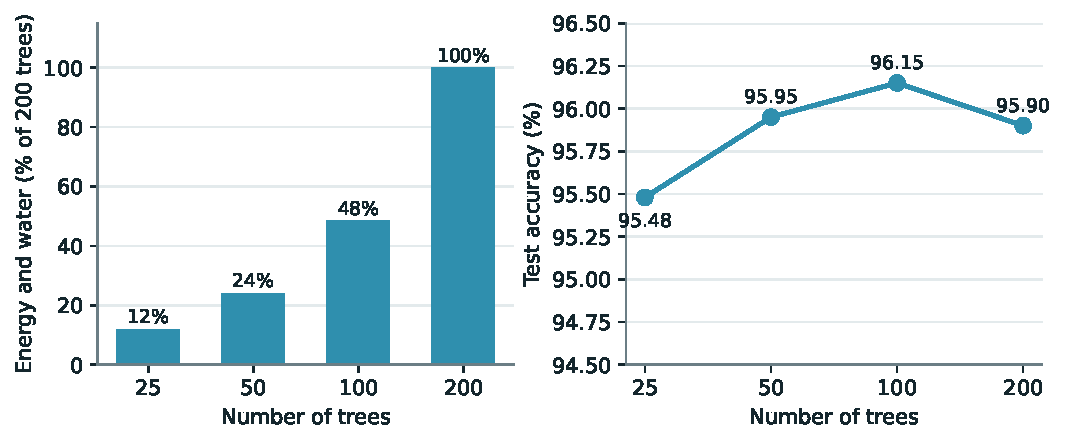
\includegraphics[width=0.6\textwidth]{figures/fig3_model_size.pdf}
\caption{Energy and water relative to 200 trees (left) and test accuracy (right). The accuracy axis spans 2 percentage points.}
\label{fig:trees}
\end{figure*}

\section{Discussion}

\textit{The grid matters more than the cooling.} The on-site share of the total is at most 22\% (Arizona), at most 20\% in every other region, and 1.5\% in the Netherlands (Table~\ref{tab:factors}). A more efficient cooling system would therefore change little for most regions, while the grid supplying the electricity changes a lot. Washington's high value comes from its EWIF of 9.501~L/kWh, not from cooling: its on-site share is 8\%.

\textit{Litres and scarcity point in different directions.} Ireland is lowest on both measures. Texas has the second-lowest footprint (0.113~mL) but High baseline water stress (3.33). Washington has the highest footprint but only Low--Medium stress (1.20). Arizona is high on both: 0.446~mL at Extremely High stress (4.39). A ranking by litres alone would favour Texas and would not separate Arizona from Sweden, which use similar litres at opposite ends of the stress scale. This is why we report both measures and do not merge them into one score.

\textit{Where the water is taken matters.} On-site water is taken at the facility, so the facility region's stress applies directly. Off-site water is taken at the power plants, which may lie in a different basin. We assign the facility region's stress to both parts, which is an approximation.

\textit{Two levers for a developer.} Choosing a region is often fixed by latency, law or cost. Choosing a model size is not: in our experiment, halving the forest from 200 to 100 trees halved the water in every region without any loss in accuracy. A developer who cannot move a job can still shrink it.

\textit{Scale.} A 5-second job is a fraction of a millilitre. The result is linear in energy, so the same factors apply to larger jobs: one million runs of this job would need about 106~L in Ireland and 708~L in Washington. The contribution of this work is the method and the comparison across regions, not the absolute size of the number.

\section{Limitations}

\begin{itemize}
\item \textit{Energy is estimated, not measured.} It rests on a nominal base power (45~W), an assumed idle power (5~W) and a linear power model. The processor can draw up to 95~W for short periods, so the true value may be higher or lower. The \pm{} values cover only run-to-run variation; no sensitivity analysis has been run yet.
\item \textit{Laptop, system-wide measurement.} Utilisation includes every process on the laptop, and data-center water factors are applied to laptop energy. This illustrates the method; it does not describe how a server would run the job.
\item \textit{Annual average factors.} WUE, PUE and EWIF are annualised values. They do not capture weather, season or time of day, although on-site WUE depends on outside temperature and humidity~\cite{li2023thirsty}.
\item \textit{One workload, one machine, one dataset.} The sets are sensitive to the thermal state of the processor and to the order of runs. Excluding Set~2 is a documented judgement, not a proven cause. The accuracy comparison uses one fixed train/test split.
\item \textit{Water stress is unvalidated and coarse.} The Aqueduct documentation states that its indicators cannot be measured directly, have not been validated, and do not model interbasin transfers. Country and state averages give different resolution across regions.
\item \textit{Scope.} Embodied (scope~3) water and the 7 projected regions of~\cite{li2023thirsty} are excluded.
\end{itemize}

\section{Conclusion and Future Work}

WattToWater turns the energy of a software job into litres of on-site and off-site water and shows them next to the water stress of each region. Three findings stand out for this job: the region changes the footprint 6.7-fold, the electricity grid and not the cooling system drives most of it, and the cheapest region in litres can sit in a water-stressed basin. A developer who cannot change the region can still halve the water by choosing a smaller model at the same accuracy.

Future work will (i)~replace the estimated power with a measured value from a wall meter or hardware sensor; (ii)~add a sensitivity analysis over base power, idle power and the regional factors, and its effect on the ranking of regions; (iii)~measure more workloads, including GPU workloads; (iv)~test whether time of day matters, using weather-dependent on-site WUE and hourly grid data once such a model is validated; and (v)~replace country and state averages with basin-level water stress and established water-scarcity footprint methods.

\section*{Data and Code Availability}

All measurements, the library and the scripts behind every number, table and figure are at \url{https://github.com/gozdegonul/WattToWater}; \texttt{analysis.py} regenerates them from the recorded runs. An interactive water map is at \url{https://gozdegonul.github.io/WattToWater/}.

\begin{thebibliography}{00}
\bibitem{li2023thirsty} P. Li, J. Yang, M. A. Islam, and S. Ren, ``Making AI less `thirsty': Uncovering and addressing the secret water footprint of AI models,'' arXiv:2304.03271, v5, Mar. 2025. [Online]. Available: \url{https://arxiv.org/abs/2304.03271}
\bibitem{wri2023aqueduct} World Resources Institute, ``Aqueduct 4.0 country rankings,'' dataset, file Aqueduct40\_rankings\_download\_Y2023M07D05.xlsx, 2023. Technical note: doi:10.46830/writn.23.00061.
\bibitem{intel12450h} Intel Corporation, ``Intel Core i5-12450H processor (12M cache, up to 4.40 GHz): Product specifications.'' [Online]. Available: \url{https://www.intel.com/content/www/us/en/products/sku/132222/intel-core-i512450h-processor-12m-cache-up-to-4-40-ghz/specifications.html} (accessed Nov. 17, 2026).
\bibitem{pedregosa2011sklearn} F. Pedregosa \textit{et al.}, ``Scikit-learn: Machine learning in Python,'' \textit{J. Mach. Learn. Res.}, vol. 12, pp. 2825--2830, 2011.
\bibitem{psutil} G. Rodola, ``psutil: Cross-platform lib for process and system monitoring in Python,'' version 7.2.2. [Online]. Available: \url{https://github.com/giampaolo/psutil}
\end{thebibliography}

\end{document}
